\section{mr::infobuffer Struct Reference}
\label{structmr_1_1infobuffer}\index{mr::infobuffer@{mr::infobuffer}}
{\tt \#include $<$mr\-Stream.h$>$}

Inheritance diagram for mr::infobuffer::\begin{figure}[H]
\begin{center}
\leavevmode
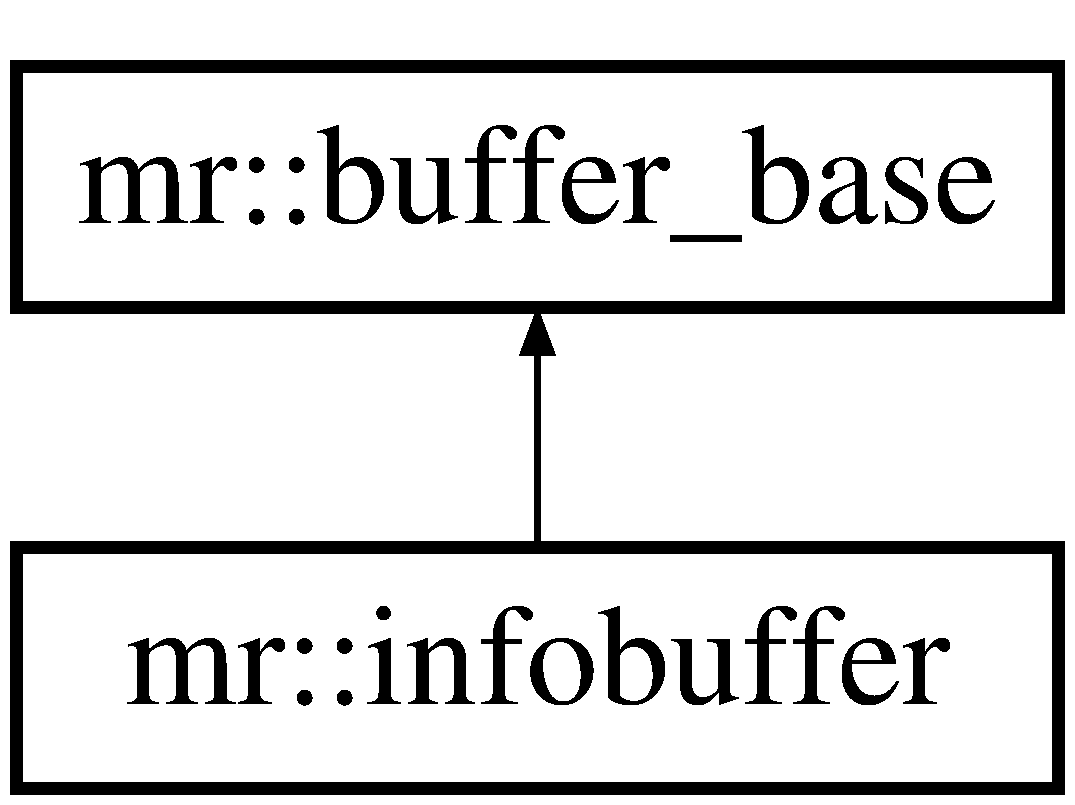
\includegraphics[height=2cm]{structmr_1_1infobuffer}
\end{center}
\end{figure}
\subsection*{Public Member Functions}
\begin{CompactItemize}
\item 
{\bf infobuffer} ()
\item 
virtual void {\bf print} (const char $\ast$const s)
\begin{CompactList}\small\item\em virtual function to print string out \item\end{CompactList}\end{CompactItemize}


\subsection{Detailed Description}
mental ray's printing out to console is based on old printf() syntax. This file uses some C++ wizardry to create some streams for printing out.

That is, instead of: mi\-Vector v; mi\_\-info(\char`\"{}[\%f, \%f, \%f] hello\char`\"{}, v.x, v.y, v.z);

you just can do: mr\_\-info( v $<$$<$ \char`\"{} hello\char`\"{} ); 



\subsection{Constructor \& Destructor Documentation}
\index{mr::infobuffer@{mr::infobuffer}!infobuffer@{infobuffer}}
\index{infobuffer@{infobuffer}!mr::infobuffer@{mr::infobuffer}}
\subsubsection{\setlength{\rightskip}{0pt plus 5cm}mr::infobuffer::infobuffer ()\hspace{0.3cm}{\tt  [inline]}}\label{structmr_1_1infobuffer_a0}




\subsection{Member Function Documentation}
\index{mr::infobuffer@{mr::infobuffer}!print@{print}}
\index{print@{print}!mr::infobuffer@{mr::infobuffer}}
\subsubsection{\setlength{\rightskip}{0pt plus 5cm}virtual void mr::infobuffer::print (const char $\ast$const {\em s})\hspace{0.3cm}{\tt  [inline, virtual]}}\label{structmr_1_1infobuffer_a1}


virtual function to print string out 



Implements {\bf mr::buffer\_\-base} {\rm (p.\,\pageref{structmr_1_1buffer__base_a3})}.

The documentation for this struct was generated from the following file:\begin{CompactItemize}
\item 
{\bf mr\-Stream.h}\end{CompactItemize}
